
%%%%%%%%%%%%%%%%%%%%%%% file typeinst.tex %%%%%%%%%%%%%%%%%%%%%%%%%
%
% This is the LaTeX source for the instructions to authors using
% the LaTeX document class 'llncs.cls' for contributions to
% the Lecture Notes in Computer Sciences series.
% http://www.springer.com/lncs       Springer Heidelberg 2006/05/04
%
% It may be used as a template for your own input - copy it
% to a new file with a new name and use it as the basis
% for your article.
%
% NB: the document class 'llncs' has its own and detailed documentation, see
% ftp://ftp.springer.de/data/pubftp/pub/tex/latex/llncs/latex2e/llncsdoc.pdf
%
%%%%%%%%%%%%%%%%%%%%%%%%%%%%%%%%%%%%%%%%%%%%%%%%%%%%%%%%%%%%%%%%%%%


\documentclass[runningheads,a4paper]{llncs}

\usepackage{amssymb}
\setcounter{tocdepth}{3}
\usepackage{graphicx}

\usepackage{url}
\newcommand{\keywords}[1]{\par\addvspace\baselineskip
\noindent\keywordname\enspace\ignorespaces#1}

\usepackage{mathtools}
\usepackage{dsfont}
\usepackage{booktabs}
\usepackage{caption}
\usepackage{subfig}
%\usepackage{subcaption}
%\captionsetup{compatibility=false}

\DeclareMathOperator*{\argmin}{arg\,min}
\DeclareMathOperator*{\argmax}{arg\,max}

\usepackage{expl3}
\ExplSyntaxOn
\newcommand\latinabbrev[1]{
  \peek_meaning:NTF . {% Same as \@ifnextchar
    #1\@}%
  { \peek_catcode:NTF a {% Check whether next char has same catcode as \'a, i.e., is a letter
      #1.\@ }%
    {#1.\@}}}
\ExplSyntaxOff

%Omit final dot from each def.
\def\eg{\latinabbrev{e.g}}
\def\etal{\latinabbrev{et al}}
\def\etc{\latinabbrev{etc}}
\def\ie{\latinabbrev{i.e}}
\def\aka{\latinabbrev{a.k.a}}

\newcommand{\Epsilon}{E}

\begin{document}

\mainmatter  % start of an individual contribution

% first the title is needed
\title{Experimental Report on Fixed-Budget Best Arm Identification}

% a short form should be given in case it is too long for the running head
\titlerunning{BAI Report}

% the name(s) of the author(s) follow(s) next
%
% NB: Chinese authors should write their first names(s) in front of
% their surnames. This ensures that the names appear correctly in
% the running heads and the author index.
%
\author{\textbf{Xuedong Shang}}
%
\authorrunning{Xuedong Shang}
% (feature abused for this document to repeat the title also on left hand pages)

% the affiliations are given next; don't give your e-mail address
% unless you accept that it will be published
%\institute{Universit\'e de Rennes 1, Parcours MRI \\ \email{xuedong.shang@ens-rennes.fr}}

%
% NB: a more complex sample for affiliations and the mapping to the
% corresponding authors can be found in the file "llncs.dem"
% (search for the string "\mainmatter" where a contribution starts).
% "llncs.dem" accompanies the document class "llncs.cls".
%

\toctitle{}
\tocauthor{Xuedong Shang}
\maketitle


\begin{abstract}

\end{abstract}


\section{Introduction}

We consider here some fixed-budget and anytime best arm identification algorithms, including Uniform Allocation~\cite{bubeck2009}, UCB-E~\cite{audibert2010}, Successive Reject~\cite{audibert2010}, fixed-budget version of UGapE~\cite{gabillon2012},  Sequential Halving~\cite{karnin2013}, Thompson Sampling coupled with MPA, Top-Two Thompson Sampling and Top-Two Probability Sampling~\cite{russo2016}, AT-LUCB~\cite{jun2016}.

\paragraph{\bfseries{Acronyme}} 
\begin{itemize}
	\item $\operatorname{EDP} = $ Empirical Distribution of Plays
	\item $\operatorname{EBA} = $ Empirical Best Arm
	\item $\operatorname{MPA} = $ Most Played Arm
	\item $\operatorname{SR} = $ Successive Reject
	\item $\operatorname{SHA} = $ Sequential Halving
	\item $\operatorname{TS} = $ Thompson Sampling
	\item $\operatorname{TTTS} = $ Top-Two Thompson Sampling
	\item $\operatorname{TTPS} = $ Top-Two Probability Sampling
	\item $\operatorname{UCB} = $ Upper Confidence Bound
	\item $\operatorname{LCB} = $ Lower Confidence Bound
\end{itemize}

\section{Comparison of Different Algorithms}

\paragraph{\bfseries{Experimental Settings}}
We use 7 problem instances proposed by~\cite{audibert2010} $+$ one hand-made simple problem instance, all settings consider only Bernoulli distributions for the moment (remark that setting 8 below is the same setting as setting 7, but only has a larger budget):
\begin{itemize}
	\item Setting 0: $\mathbf{\mu}=[0.4, 0.5, 0.35, 0.3], \operatorname{budget}=1000$
	\item Setting 1: $\mathbf{\mu_1}=0.5, \mathbf{\mu_{2:20}}=0.4, \operatorname{budget}=2000$
	\item Setting 2: $\mathbf{\mu_1}=0.5, \mathbf{\mu_{2:6}}=0.42, \mathbf{\mu_{7:20}}=0.38, \operatorname{budget}=2000$
	\item Setting 3: $\mathbf{\mu}=[0.5, 0.3631, 0.449347, 0.48125839], \operatorname{budget}=2000$
	\item Setting 4: $\mathbf{\mu}=[0.5, 0.42, 0.4, 0.4, 0.35, 0.35], \operatorname{budget}=600$
	\item Setting 5: $\mathbf{\mu_1}=0.5, \mathbf{\mu_i}=\mathbf{\mu_1}-0.025i, \forall i\in\{2\ldots15\}, \operatorname{budget}=4000$
	\item Setting 6: $\mathbf{\mu_1}=0.5, \mathbf{\mu_2}=0.48, \mathbf{\mu_{3:20}}=0.37, \operatorname{budget}=6000$
	\item Setting 7: $\mathbf{\mu_1}=0.5, \mathbf{\mu_{2:6}}=0.45, \mathbf{\mu_{7:20}}=0.43, \mathbf{\mu_{7:20}}=0.38, \operatorname{budget}=6000$
	\item Setting 8: $\mathbf{\mu_1}=0.5, \mathbf{\mu_{2:6}}=0.45, \mathbf{\mu_{7:20}}=0.43, \mathbf{\mu_{7:20}}=0.38, \operatorname{budget}=12000$
\end{itemize}

\paragraph{\bfseries{Some Implementation Details}}
All algorithms are implemented in Julia.
\begin{itemize}
	\item UCB-E: UCB-E has two versions of implementations, where the adaptive version estimates online the parameter $H_1$. And we use EBA as recommendation strategy for UCB-E in this section.
	\item SR: In SR we need to pay a little attention. Indeed, we need to use \textit{Round-Robin} when we pull arms in each elimination phase. For the moment, we also use EBA as recommendation strategy.
	\item UGapE: UGapE also faces the problem of unknown $H_1$ parameter, thus we also have an adaptive version of the algorithm. Note that UGapE has its own recommendation strategy which is not included in EBA, EDP and MPA.
	\item SHA: SHA also has two versions of implementations. The first one which I call \textit{SHA with Refresh} means that at each elimination phase, we will discard the statistics of each arm we obtained from previous elimination rounds. While the second one which I call \textit{SHA without Refresh} means that we will keep the statistics at each elimination phase. Note that we also need to use Round-Robin when we pull arms in each elimination phase as in SR. The recommendation strategy is also EBA here.
	\item AT-LUCB: The recommendation strategy of AT-LUCB is also a bit of different from other algorithms. Since it's a LUCB-type algorithm, we need to pull two arms (one based on UCBs and one based on LCBs), thus at each time step we will recommend two times the same arm using EBA strategy.
	\item TS with MPA: In TS, we draw parameter samples from the posterior instead of computing the optimal action probabilities, since the latter one requires a much larger computational effort.
\end{itemize}

\paragraph{\bfseries{Thompson Sampling with MPA}}
In this part, all the plots are averaged on 10000 trials of experiments and we plot the trend of simple regret for each algorithm. In this part we include only Uniform Sampling, UCB-E, SR, UGapE, SHA, AT-LUCB and TS with MPA. The objective is to see how TS with MPA performs compared to state-of-the-art fixed-budget algorithms.

\begin{figure}[ht]
	\centering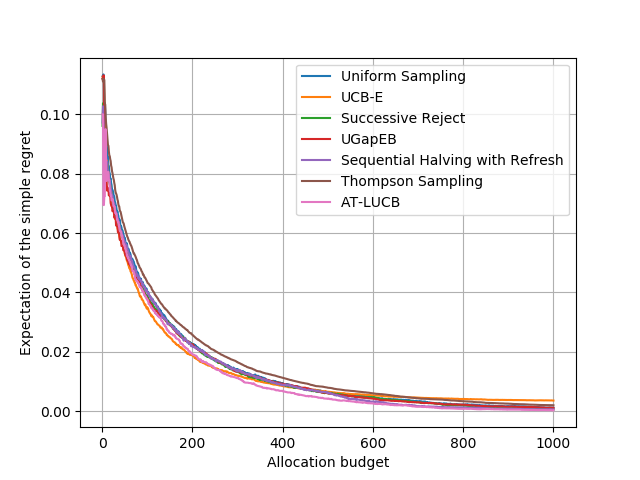
\includegraphics[width=\textwidth]{../results/ts_mpa/setting0.png}
    	\caption{Problem Setting 0}
	\label{ts_mpa_0}
\end{figure}
\begin{figure}[ht]
    	\centering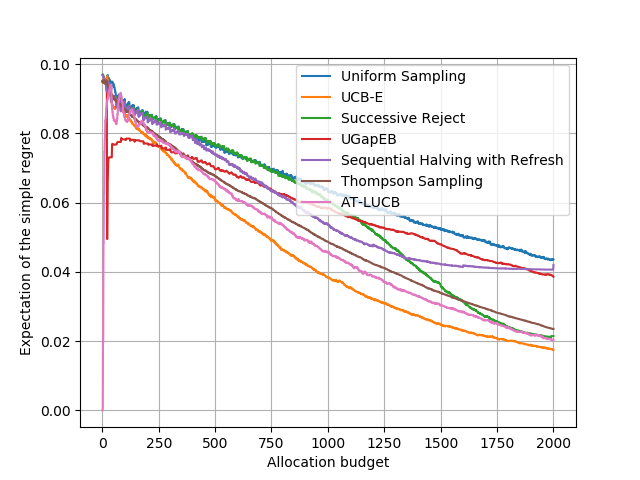
\includegraphics[width=\textwidth]{../results/ts_mpa/setting1.png}
    	\caption{Problem Setting 1}
	\label{ts_mpa_1}
\end{figure}
\begin{figure}[ht]
   	\centering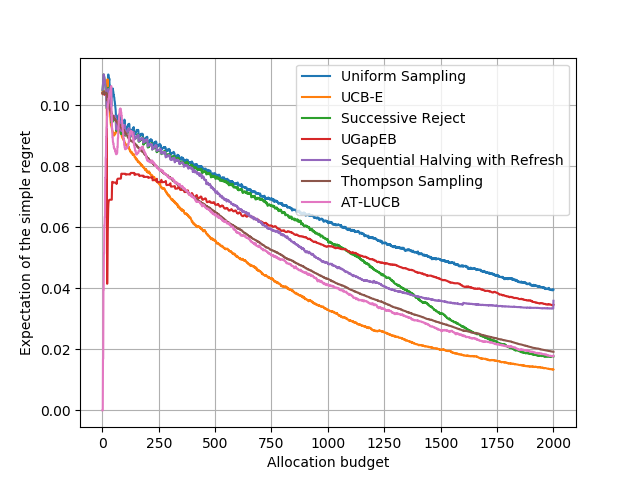
\includegraphics[width=\textwidth]{../results/ts_mpa/setting2.png}
   	 \caption{Problem Setting 2}
	\label{ts_mpa_2}
\end{figure}
\begin{figure}[ht]
    	\centering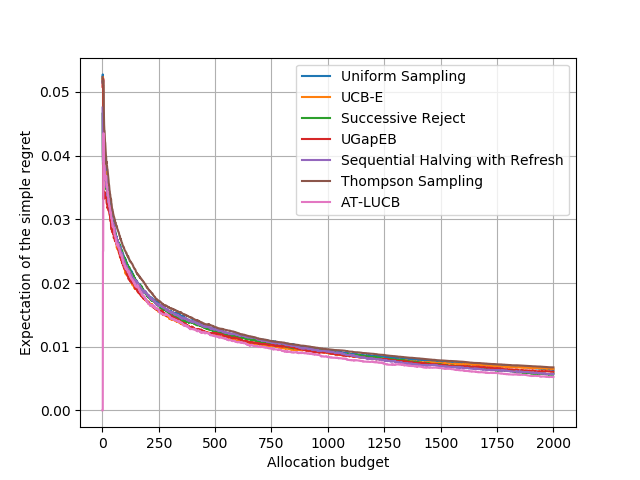
\includegraphics[width=\textwidth]{../results/ts_mpa/setting3.png}
    	\caption{Problem Setting 3}
	\label{ts_mpa_3}
\end{figure}
\begin{figure}[ht]
    	\centering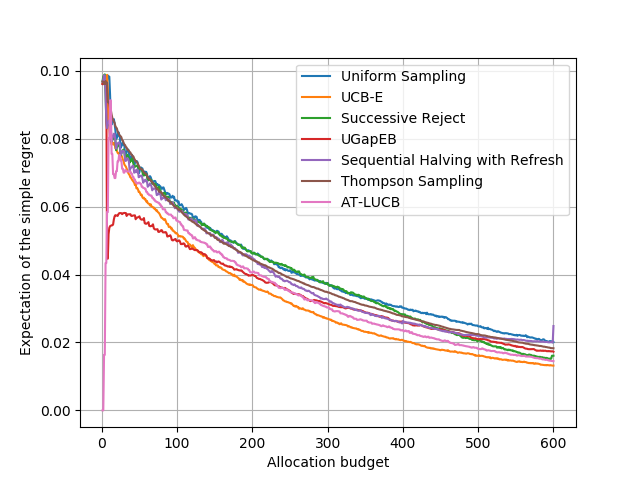
\includegraphics[width=\textwidth]{../results/ts_mpa/setting4.png}
    	\caption{Problem Setting 4}
	\label{ts_mpa_4}
\end{figure}
\begin{figure}[ht]
	\centering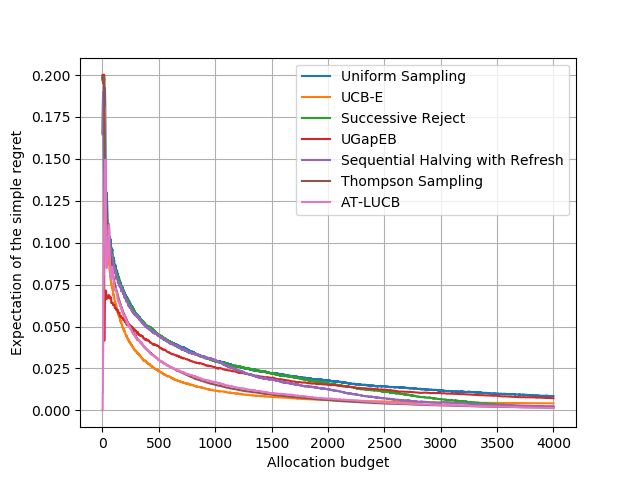
\includegraphics[width=\textwidth]{../results/ts_mpa/setting5.png}
    	\caption{Problem Setting 5}
	\label{ts_mpa_5}
\end{figure}
\begin{figure}[ht]
    	\centering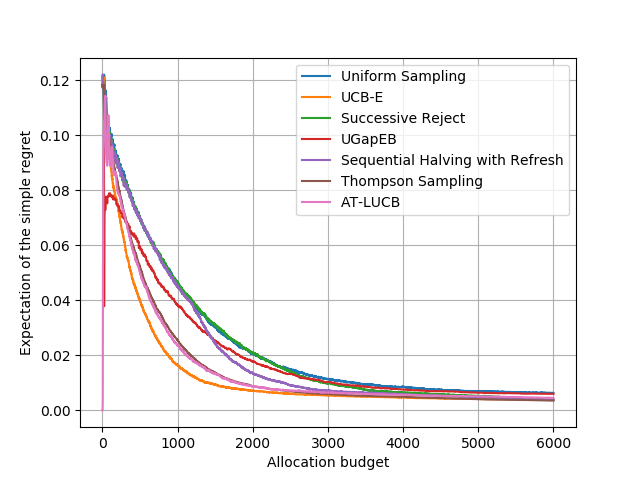
\includegraphics[width=\textwidth]{../results/ts_mpa/setting6.png}
    	\caption{Problem Setting 6}
	\label{ts_mpa_6}
\end{figure}
\begin{figure}[ht]
   	\centering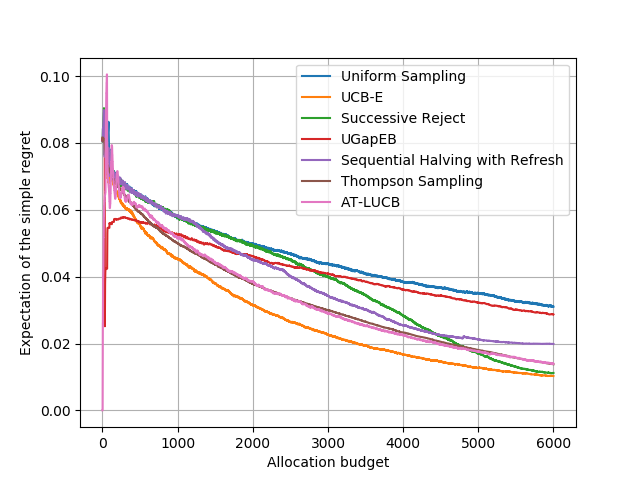
\includegraphics[width=\textwidth]{../results/ts_mpa/setting7.png}
   	 \caption{Problem Setting 7}
	\label{ts_mpa_7}
\end{figure}
\begin{figure}[ht]
    	\centering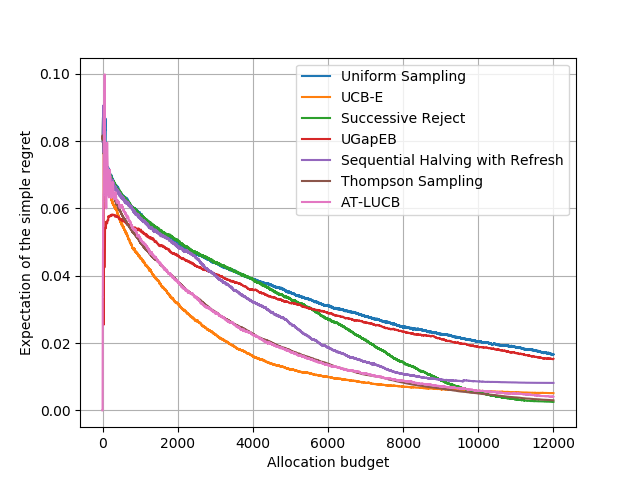
\includegraphics[width=\textwidth]{../results/ts_mpa/setting8.png}
    	\caption{Problem Setting 8}
	\label{ts_mpa_8}
\end{figure}

From Fig.~\ref{ts_mpa_5} to~\ref{ts_mpa_8} we can see that TS with MPA performs almost as well as AT-LUCB, and beats other algorithms (note that we don't really take into account UCB-E which seems to be always the best, since we cannot know $H_1$ in advance). These are actually some relatively difficulty problem instances in this report.

TODO: log-scale figures.

\paragraph{\bfseries{Top-Two Thompson Sampling and Top-Two Probability Sampling}}
For TTTS and TTPS, we now need to compute the optimal action probabilities. Actually, in the original TTTS algorithm, we don't need to compute these probabilities since we can always use the parameter sampling from the posterior trick. However, since we are now in a best arm identification setting, and a plausible recommendation strategy for TTTS and TTPS would be recommending at each time step the arm with the largest optimal action probability. Thus in both cases, we need to compute these probabilities. And in practice, we use the Cubature package of Julia to complete this task.

\begin{figure}%
    \centering
    \subfloat[linear scale]{{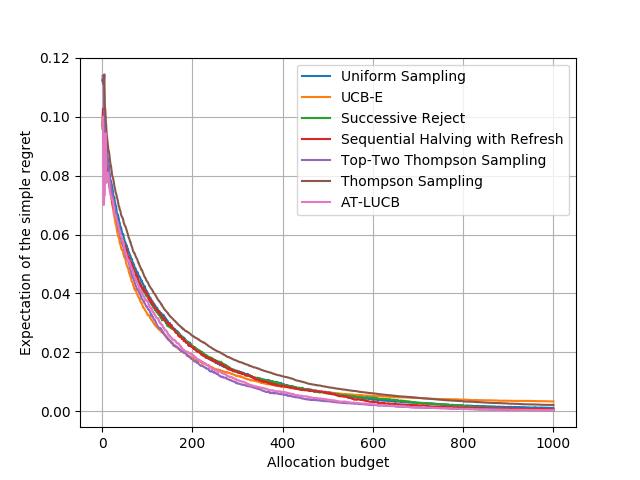
\includegraphics[width=5cm]{../results/ttts/setting0.png} }}%
    \qquad
    \subfloat[log scale]{{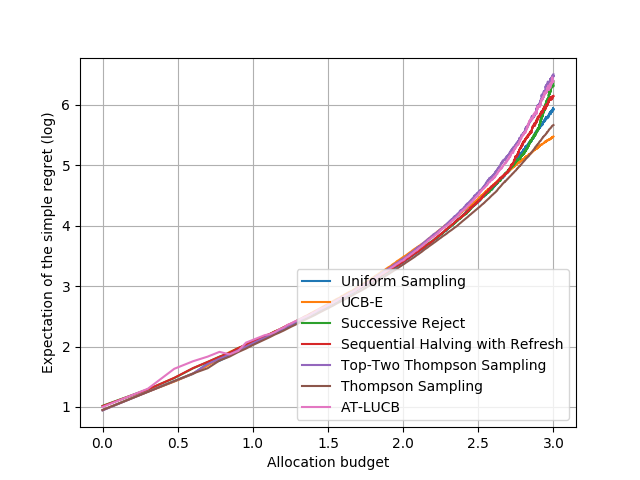
\includegraphics[width=5cm]{../results/ttts/setting0_log.png} }}%
    \caption{Problem Setting 0}%
    \label{ttts_0}%
\end{figure}
\begin{figure}%
    \centering
    \subfloat[linear scale]{{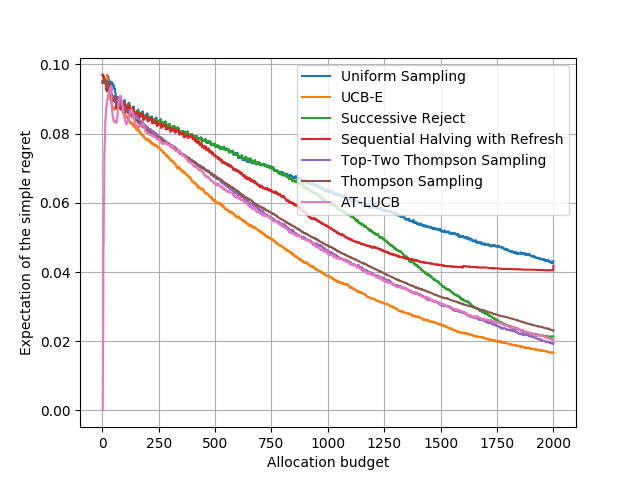
\includegraphics[width=5cm]{../results/ttts/setting1.png} }}%
    \qquad
    \subfloat[log scale]{{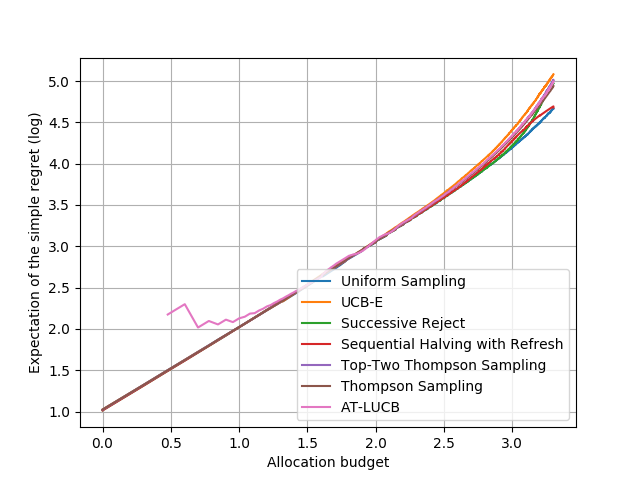
\includegraphics[width=5cm]{../results/ttts/setting1_log.png} }}%
    \caption{Problem Setting 1}%
    \label{ttts_1}%
\end{figure}
\begin{figure}%
    \centering
    \subfloat[linear scale]{{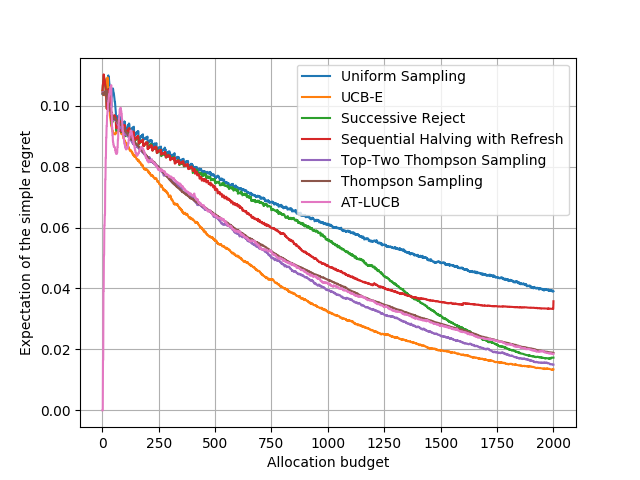
\includegraphics[width=5cm]{../results/ttts/setting2.png} }}%
    \qquad
    \subfloat[log scale]{{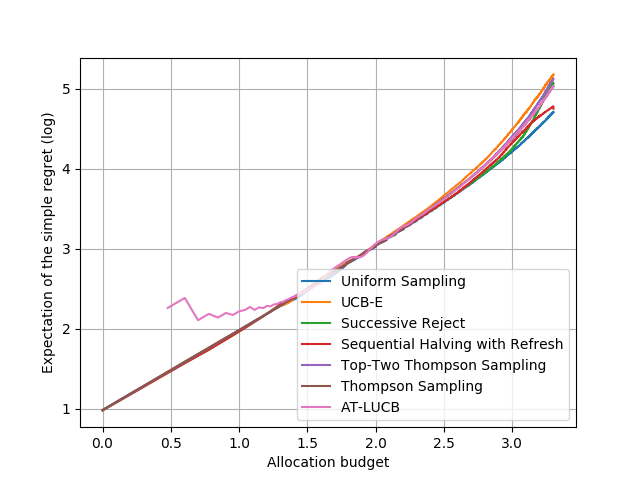
\includegraphics[width=5cm]{../results/ttts/setting2_log.png} }}%
    \caption{Problem Setting 2}%
    \label{ttts_2}%
\end{figure}
\begin{figure}%
    \centering
    \subfloat[linear scale]{{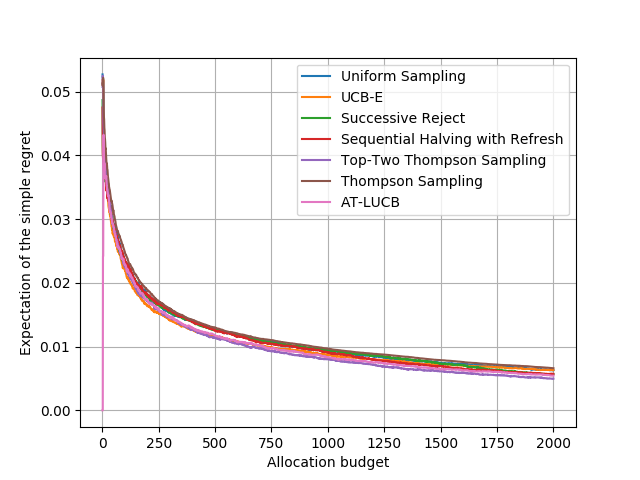
\includegraphics[width=5cm]{../results/ttts/setting3.png} }}%
    \qquad
    \subfloat[log scale]{{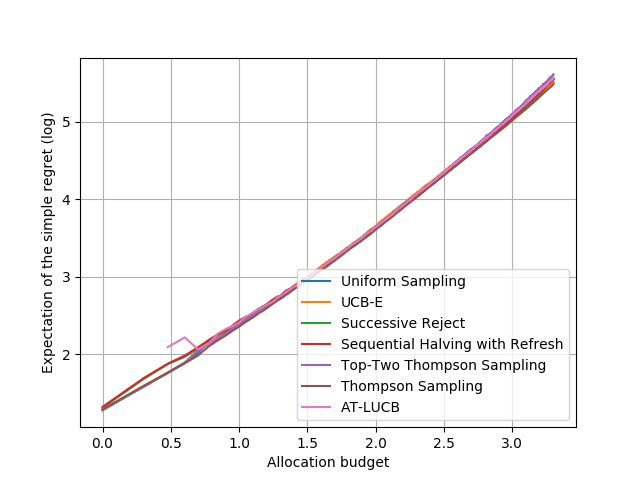
\includegraphics[width=5cm]{../results/ttts/setting3_log.png} }}%
    \caption{Problem Setting 3}%
    \label{ttts_3}%
\end{figure}
\begin{figure}%
    \centering
    \subfloat[linear scale]{{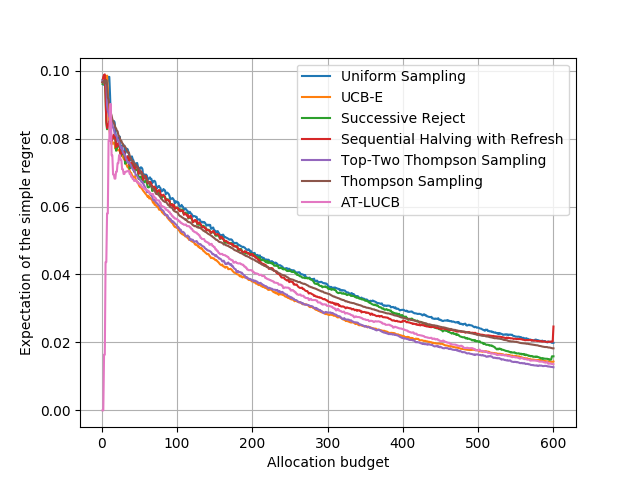
\includegraphics[width=5cm]{../results/ttts/setting4.png} }}%
    \qquad
    \subfloat[log scale]{{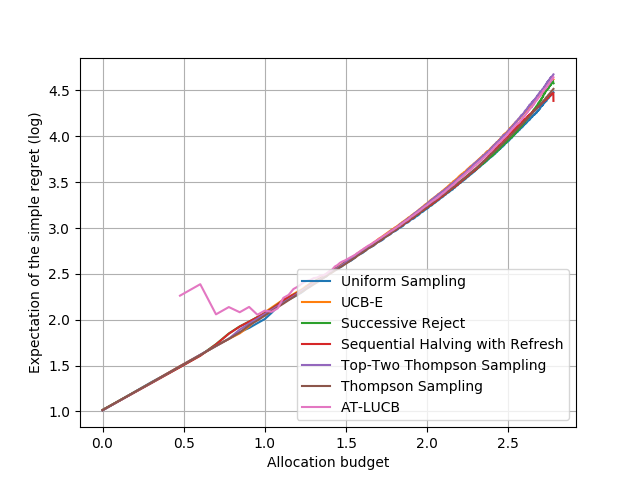
\includegraphics[width=5cm]{../results/ttts/setting4_log.png} }}%
    \caption{Problem Setting 4}%
    \label{ttts_4}%
\end{figure}
\begin{figure}%
    \centering
    \subfloat[linear scale]{{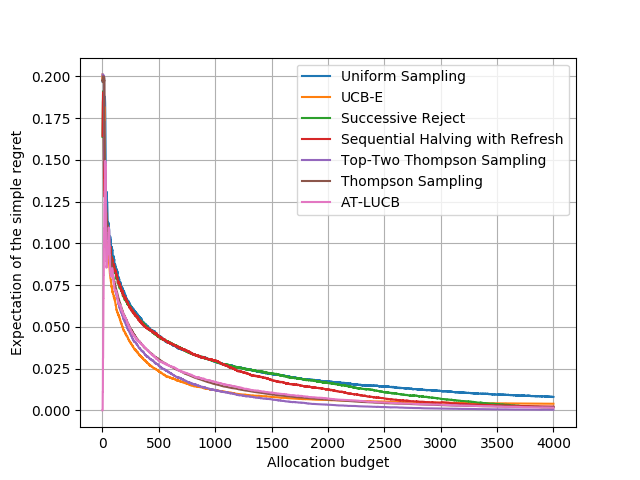
\includegraphics[width=5cm]{../results/ttts/setting5.png} }}%
    \qquad
    \subfloat[log scale]{{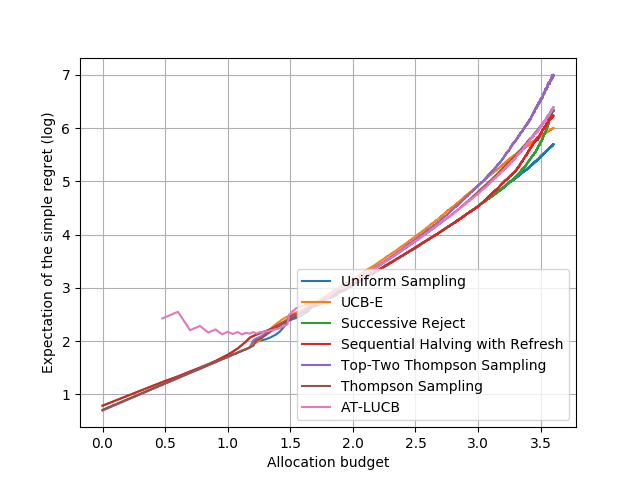
\includegraphics[width=5cm]{../results/ttts/setting5_log.png} }}%
    \caption{Problem Setting 5}%
    \label{ttts_5}%
\end{figure}
\begin{figure}%
    \centering
    \subfloat[linear scale]{{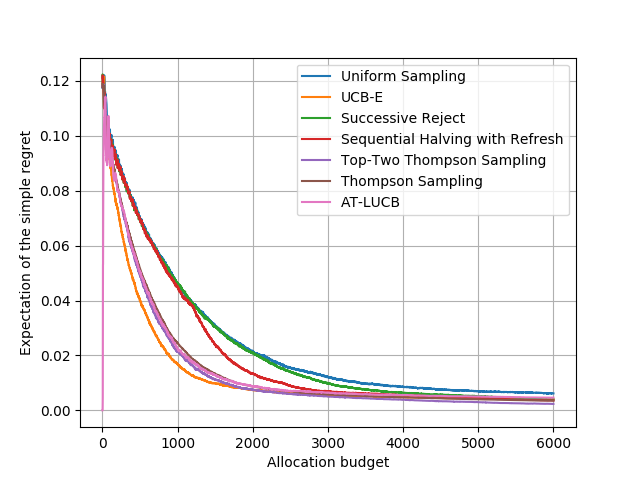
\includegraphics[width=5cm]{../results/ttts/setting6.png} }}%
    \qquad
    \subfloat[log scale]{{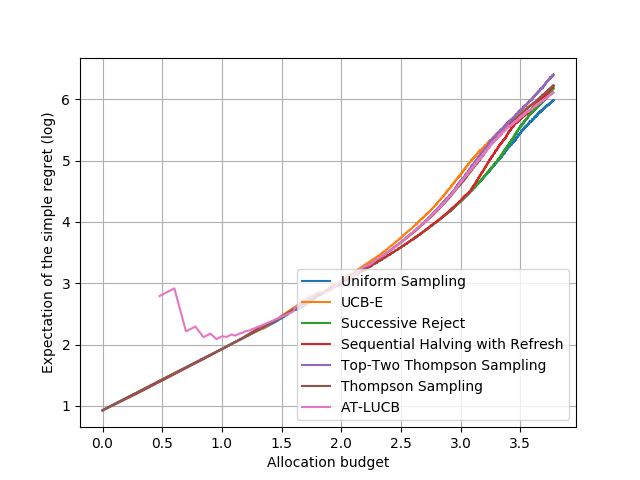
\includegraphics[width=5cm]{../results/ttts/setting6_log.png} }}%
    \caption{Problem Setting 6}%
    \label{ttts_6}%
\end{figure}
\begin{figure}%
    \centering
    \subfloat[linear scale]{{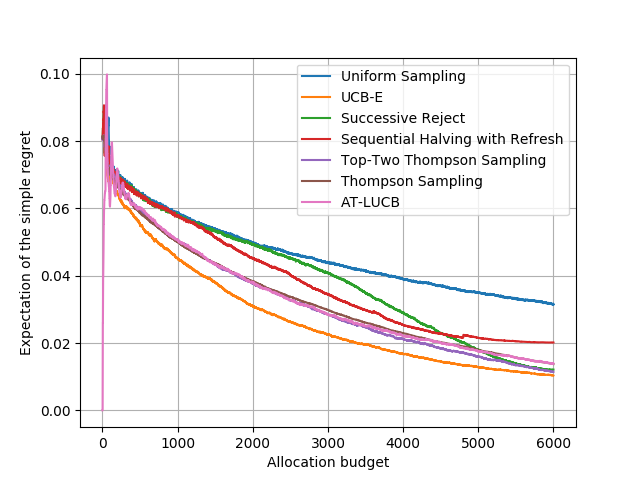
\includegraphics[width=5cm]{../results/ttts/setting7.png} }}%
    \qquad
    \subfloat[log scale]{{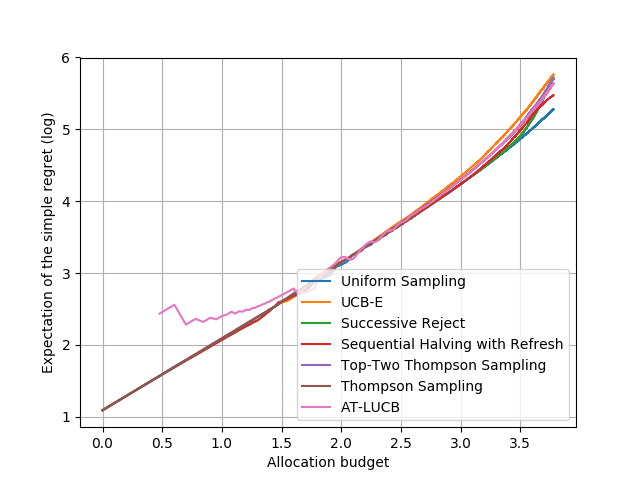
\includegraphics[width=5cm]{../results/ttts/setting7_log.png} }}%
    \caption{Problem Setting 7}%
    \label{ttts_7}%
\end{figure}
\begin{figure}%
    \centering
    \subfloat[linear scale]{{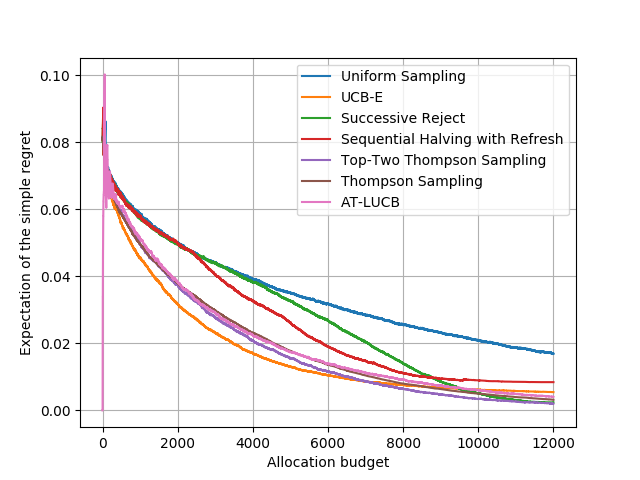
\includegraphics[width=5cm]{../results/ttts/setting8.png} }}%
    \qquad
    \subfloat[log scale]{{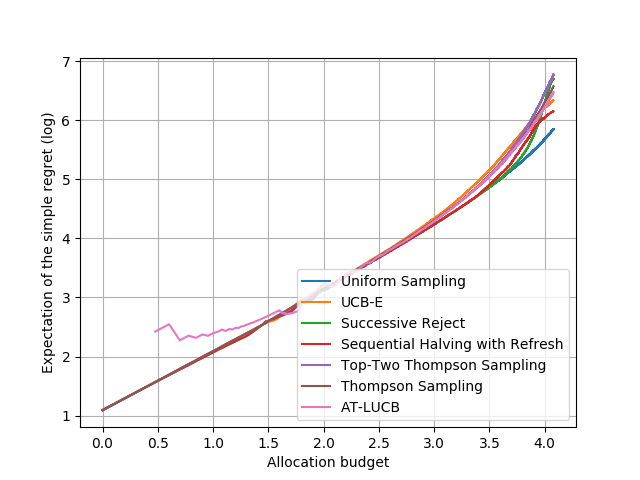
\includegraphics[width=5cm]{../results/ttts/setting8_log.png} }}%
    \caption{Problem Setting 8}%
    \label{ttts_8}%
\end{figure}

For the moment, all the plots in this part are averaged on 10000 trials. From Fig.~\ref{ttts_0} to~\ref{ttts_8} we can see that Top-Two Thompson Sampling performs almost always the best (except the cheating UCB-E).

\section{Comparison of Different Recommendation Strategies}

TODO

\begin{thebibliography}{4}

\bibitem{bubeck2009} Bubeck, S., Munos, R., \& Stoltz, G. (2009, October). Pure exploration in multi-armed bandits problems. In International conference on Algorithmic learning theory (pp. 23-37). Springer, Berlin, Heidelberg.
\bibitem{audibert2010} Audibert, J. Y., \& Bubeck, S. (2010, June). Best arm identification in multi-armed bandits. In COLT-23th Conference on Learning Theory-2010 (pp. 13-p).
\bibitem{gabillon2012} Gabillon, V., Ghavamzadeh, M., \& Lazaric, A. (2012). Best arm identification: A unified approach to fixed budget and fixed confidence. In Advances in Neural Information Processing Systems (pp. 3212-3220).
\bibitem{karnin2013} Karnin, Z., Koren, T., \& Somekh, O. (2013, February). Almost optimal exploration in multi-armed bandits. In International Conference on Machine Learning (pp. 1238-1246).
\bibitem{russo2016} Russo, D. (2016, June). Simple bayesian algorithms for best arm identification. In Conference on Learning Theory (pp. 1417-1418).
\bibitem{jun2016} Jun, K. S., \& Nowak, R. D. (2016, June). Anytime Exploration for Multi-armed Bandits using Confidence Information. In ICML (pp. 974-982).

\end{thebibliography}


%\section*{Appendix}

\end{document}
